\chapter{Введение в проблему. Исторический обзор}\label{ch:ch1}

\section{Примеры}
Критически важным (\textbf{mission-critical}) фактором системы является любой фактор
(компонент, оборудование, персонал, процесс, процедура, программное обеспечение и т. д.),
необходимый для ведения бизнеса или для организации.
Отказ или срыв одного из факторов приведет к серьезному воздействию на бизнес-операции или на организацию
и даже может вызвать социальные потрясения и катастрофы.

Приведем примеры катастроф, приведших к человеческим жертвам, большим экономическим потерям,
по причине наличия ошибок или недочетов в программно-аппаратных комплексах.

\subsection{Ariane~5}

    Первый испытательный полет в 1996 году Ariane~5 \cite{journal:open_system:1998_adjaev}\footnote{\url{http://www.osp.ru/os/1998/06/179592}},
    европейской одноразовой тяжёлой ракеты-носителя семейства Ариан,
    предназначеной для выведения полезной нагрузки на низкую опорную орбиту или геопереходную орбиту. 
    %
    Ракета-носитель была подорвана на 34-й секунде полёта по причине неисправности в управляющем программном обеспечении.
    Конвертация данных из 64-разрядного числа с плавающей запятой в 16-разрядное привела к зависанию компьютера.
    Процедура на языке Ada, обрабатывающая эту исключительную ситуацию, была исключена из соображений сохранения производительности системы.
    %
    Это считается самой дорогостоящей компьютерной ошибкой в истории.
    Отметим, что всю цепь событий удалось полностью воспроизвести с помощью компьютерного \textbf{моделирования}, что вкупе с материалами других исследований и экспериментов позволило полностью выявить причины и обстоятельства катастрофы.
    %
    %
\subsection{Therac-25}

    Аппарат лучевой терапии Therac-25 стал причиной как минимум шести передозировок радиации (июнь 1985 --- январь 1987 гг.),
    некоторые пациенты получили дозы в десятки тысяч рад. Как минимум двое умерли непосредственно от передозировок \cite{journal:computer:1993:therac25}.
    Внешний вид прибора показан на рисунке \ref{fig:therac25}.
    %
    %
\subsection{Блэкоут}
    В 2003 году\footnote{\url{https://m.habr.com/ru/company/mailru/blog/370153/}}.
    %
    %
\subsection{Третья мировая война} % https://m.habr.com/ru/company/mailru/blog/485612
    Запуск балистических ракет в 1983 году (там же).
    %
    %
    \subsection{Перелет через линию смены дат}
    Смена часового пояса у истребителей F-22. 

\begin{center}
\begin{figure}[hb]
    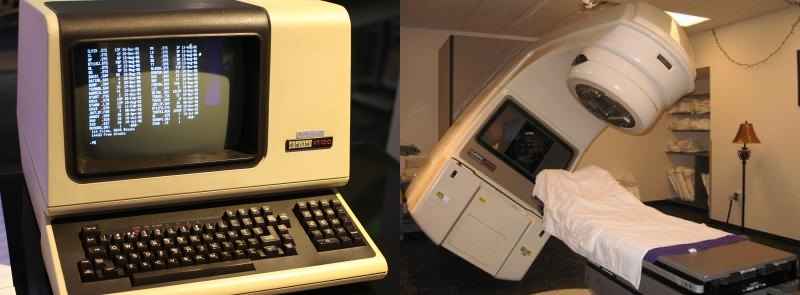
\includegraphics[width=.7\textwidth]{therac25-console}
    \caption{Therac 25}\label{fig:therac25}
    %
    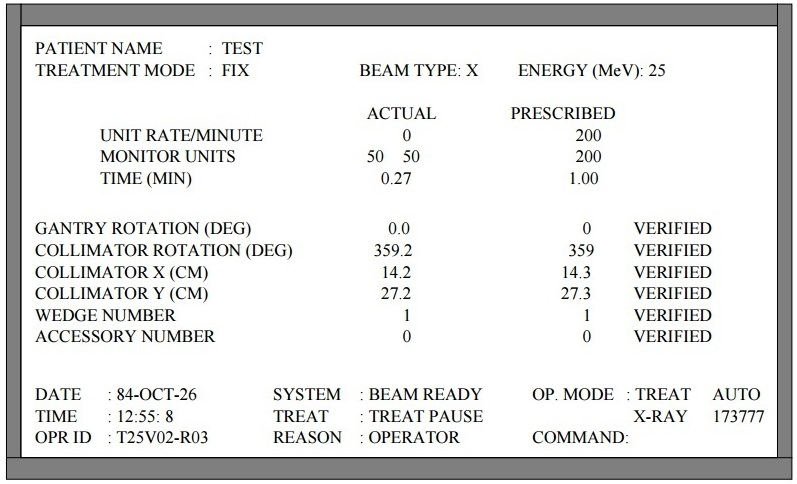
\includegraphics[width=.7\textwidth]{therac25-screenshot}
    \caption{Консоль Therac 25}\label{fig:therac25_console}
\end{figure}
\end{center}
